%%%%%%%%%%%%%%%%%%%%%%%%%%%%%%%%%%%%%%%%%%%%%%%%%%%%%%%%%%%%%%%%%%%%%%%%%%%
% Chapter: Networking (TCP/IP)
% Reference platform: ESP32-C3 (RISC-V, Wi-Fi), simulated in Wokwi.
% Examples: examples/networking/esp32-c (Arduino, browser),
% examples/networking/esp32-rust (esp-hal + embassy-net, Wokwi for VS Code),
% examples/networking/host-c and host-rust (sockets on a PC or Replit).
%%%%%%%%%%%%%%%%%%%%%%%%%%%%%%%%%%%%%%%%%%%%%%%%%%%%%%%%%%%%%%%%%%%%%%%%%%%

%%%%%%%%%%%%%%%%%%%%%%%%%%%%%%%%%%%%%%%%%%%%%%%%%%%%%%%%%%%%%%%%%%%%%%%%%%%
\section{Networks in Embedded Systems}
%%%%%%%%%%%%%%%%%%%%%%%%%%%%%%%%%%%%%%%%%%%%%%%%%%%%%%%%%%%%%%%%%%%%%%%%%%%
\nsl{More and more embedded systems are connected. A heating controller reports
its state to a smartphone app, a machine sends its sensor data to a server for
predictive maintenance, a car downloads software updates over the air. In
almost all of these cases the protocols of the internet are used: IP,
TCP and UDP, and on top of them HTTP, MQTT or similar application protocols.
\newline
This chapter explains these protocols layer by layer. We use an ESP32-C3
microcontroller with integrated Wi-Fi, simulated in Wokwi. The simulator
provides a Wi-Fi access point and forwards the traffic to the real internet,
so our simulated device can talk to real servers. As in the previous chapter
every example exists in C and in Rust. The socket examples run on a PC
or on Replit.
\newpage}

\begin{description}
\item[{\rot\bf Why connect an embedded system?}]~\\[-3ex]
\bi
	\ite send measured data to a server or cloud service (monitoring, analysis)
	\ite remote control and configuration (smartphone app, web interface)
	\ite software updates over the air (OTA) -- often the most important reason
	\ite time synchronisation, communication between devices (machine to machine)
\ei
\bi
	\ite but: a microcontroller has little memory and often a battery
	\bi
		\ite a TCP/IP stack needs code and RAM: lwIP (used by ESP-IDF and Arduino) about 40\,KB code; buffers for every connection come on top
		\ite Wi-Fi transmission needs well above 100\,mA; Bluetooth Low Energy or LoRa are much more economical
		\ite every connected device can be attacked -- security is part of the design
	\ei
\ei
\os{\newpage}

\item[{\rot\bf The reference platform: ESP32-C3}]~\\[-3ex]
\bi
	\ite 32 bit RISC-V core, 160\,MHz, 400\,KB SRAM, 4\,MB flash on typical modules
	\ite Wi-Fi 802.11 b/g/n (2.4\,GHz) and Bluetooth LE 5 on the chip
	\ite the radio is controlled by a driver with closed-source parts supplied by Espressif
	\ite software stacks
	\bi
		\ite C: Arduino core or ESP-IDF, both with lwIP as TCP/IP stack and FreeRTOS
		\ite Rust: \texttt{esp-hal} + \texttt{esp-radio} (Wi-Fi driver) + \texttt{embassy-net} (TCP/IP stack based on smoltcp)
	\ei
	\ite in Wokwi the device connects to the open access point \textbf{Wokwi-GUEST}; the simulator routes its packets to the internet
	\bi
		\ite outgoing connections work (DNS, HTTP, MQTT, NTP); ping (ICMP) does not
		\ite incoming connections to a server on the device need the paid private gateway or port forwarding in VS Code
	\ei
\ei
\os{\newpage}

\item[{\rot\bf Layer models}]~\\[-3ex]
\bi
	\ite communication is split into layers; each layer uses the services of the layer below and offers a service to the layer above
	\ite a layer can be replaced without changing the others (Wi-Fi instead of Ethernet, IPv6 instead of IPv4)
	\ite the \textbf{OSI model} (7 layers) is the reference for terminology; the internet uses the simpler \textbf{TCP/IP model} (4 layers)
\ei
\begin{figure}[!hbtp]
\begin{center}
\resizebox{0.85\textwidth}{!}{%
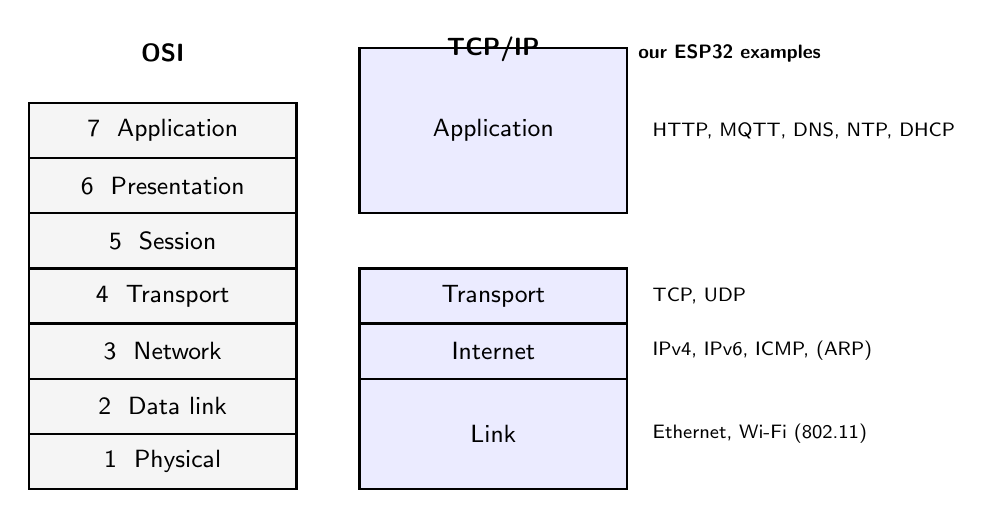
\begin{tikzpicture}[font=\sffamily\small,
	osi/.style={draw,thick,minimum width=34mm,minimum height=7mm,fill=gray!8},
	tcp/.style={draw,thick,minimum width=34mm,fill=blue!8,align=center},
	ex/.style={anchor=west,font=\sffamily\scriptsize,align=left}]
	\foreach \n/\name in {7/Application,6/Presentation,5/Session,4/Transport,3/Network,2/Data link,1/Physical}
		\node[osi] (o\n) at (0,{(\n-1)*0.7}) {\n\ \ \name};
	\node[above] at (0,4.95) {\textbf{OSI}};
	\node[tcp,minimum height=21mm] (ta) at (4.2,4.2) {Application};
	\node[tcp,minimum height=7mm] (tt) at (4.2,2.1) {Transport};
	\node[tcp,minimum height=7mm] (tn) at (4.2,1.4) {Internet};
	\node[tcp,minimum height=14mm] (tl) at (4.2,0.35) {Link};
	\node[above] at (4.2,4.95) {\textbf{TCP/IP}};
	\node[ex] at (6.1,4.2) {HTTP, MQTT, DNS, NTP, DHCP};
	\node[ex] at (6.1,2.1) {TCP, UDP};
	\node[ex] at (6.1,1.4) {IPv4, IPv6, ICMP, (ARP)};
	\node[ex] at (6.1,0.35) {Ethernet, Wi-Fi (802.11)};
	\node[above,font=\sffamily\scriptsize] at (7.2,4.95) {\textbf{our ESP32 examples}};
\end{tikzpicture}}
\caption{OSI reference model and the TCP/IP model with the protocols used in this chapter}
\end{center}
\end{figure}
\os{\newpage}

\item[{\rot\bf Encapsulation}]~\\[-3ex]
\bi
	\ite on the way down, every layer puts its own \textbf{header} in front of the data it gets from above
	\ite the receiver removes the headers layer by layer on the way up
	\ite names of the data units: message (application), segment (TCP) or datagram (UDP), packet (IP), frame (link layer)
\ei
\begin{figure}[!hbtp]
\begin{center}
\resizebox{0.9\textwidth}{!}{%
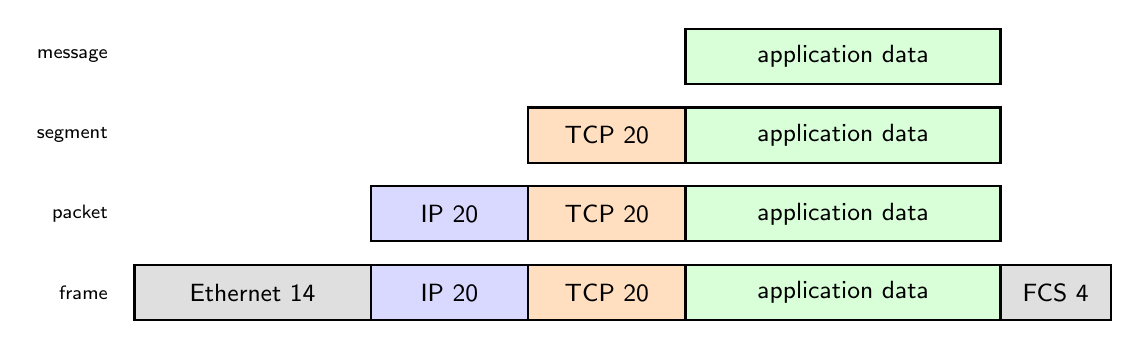
\begin{tikzpicture}[font=\sffamily\small,
	b/.style={draw,thick,minimum height=7mm,anchor=west,inner sep=2pt}]
	\newcommand{\app}[1]{\node[b,fill=green!15,minimum width=40mm] at (7,#1) {application data};}
	\newcommand{\tcp}[1]{\node[b,fill=orange!25,minimum width=20mm] at (5,#1) {TCP 20};}
	\newcommand{\ip}[1]{\node[b,fill=blue!15,minimum width=20mm] at (3,#1) {IP 20};}
	\app{3} \tcp{2} \app{2} \ip{1} \tcp{1} \app{1} \ip{0} \tcp{0} \app{0}
	\node[b,fill=gray!25,minimum width=30mm] at (0,0) {Ethernet 14};
	\node[b,fill=gray!25,minimum width=14mm] at (11,0) {FCS 4};
	\foreach \y/\t in {3/message,2/segment,1/packet,0/frame} \node[left,font=\sffamily\scriptsize] at (-0.2,\y) {\t};
\end{tikzpicture}}
\caption{Encapsulation of application data in TCP, IPv4 and Ethernet (header sizes in bytes, minimum)}
\end{center}
\end{figure}
\bi
	\ite overhead: one byte of payload costs at least $14+20+20+4 = 58$ bytes of headers on Ethernet (plus preamble and gap) -- small values should be collected and sent together
\ei
\os{\newpage}
\end{description}

%%%%%%%%%%%%%%%%%%%%%%%%%%%%%%%%%%%%%%%%%%%%%%%%%%%%%%%%%%%%%%%%%%%%%%%%%%%
\section{Link Layer: Ethernet and Wi-Fi}
%%%%%%%%%%%%%%%%%%%%%%%%%%%%%%%%%%%%%%%%%%%%%%%%%%%%%%%%%%%%%%%%%%%%%%%%%%%
\nsl{The link layer transports frames between devices that are directly
connected: over a cable to the next switch, or over radio to the access point.
It uses its own addresses, the MAC addresses, which are only meaningful
within one local network. Ethernet and Wi-Fi use the same 48 bit address
format and look the same to the layers above. This is why an IP stack does
not care whether it runs over a cable or over radio.}

\begin{description}
\item[{\rot\bf MAC addresses}]~\\[-3ex]
\bi
	\ite 48 bit, written as six bytes in hexadecimal: \texttt{24:0A:C4:00:01:10}
	\ite the first three bytes (OUI) identify the manufacturer -- 24:0A:C4 belongs to Espressif
	\ite stored in the chip (eFuse) and unique worldwide; can be overridden in software
	\ite \texttt{FF:FF:FF:FF:FF:FF} is the \textbf{broadcast} address: every device in the local network receives the frame
	\ite only valid in the local network -- a router replaces the link layer header on every hop
\ei
\os{\newpage}

\item[{\rot\bf Ethernet}]~\\[-3ex]
\begin{figure}[!hbtp]
\begin{center}
\resizebox{0.95\textwidth}{!}{%
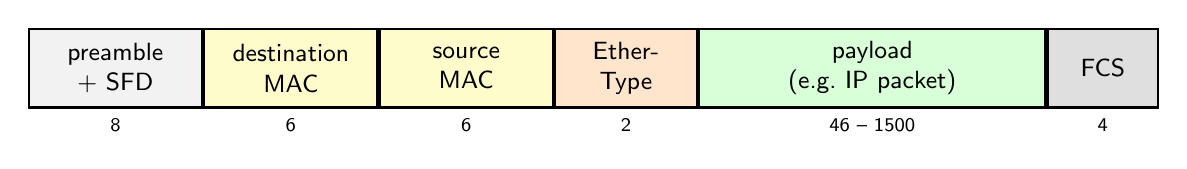
\begin{tikzpicture}[font=\sffamily\small,
	f/.style={draw,thick,minimum height=10mm,anchor=west,align=center,inner sep=1pt}]
	\node[f,fill=gray!10,minimum width=22mm] (a) at (0,0) {preamble\\+ SFD};
	\node[f,fill=yellow!20,minimum width=22mm] (b) at (a.east) {destination\\MAC};
	\node[f,fill=yellow!20,minimum width=22mm] (c) at (b.east) {source\\MAC};
	\node[f,fill=orange!20,minimum width=18mm] (d) at (c.east) {Ether-\\Type};
	\node[f,fill=green!15,minimum width=44mm] (e) at (d.east) {payload\\(e.g.\ IP packet)};
	\node[f,fill=gray!25,minimum width=14mm] (g) at (e.east) {FCS};
	\foreach \n/\s in {a/8,b/6,c/6,d/2,e/46 -- 1500,g/4} \node[below,font=\sffamily\scriptsize] at (\n.south) {\s};
\end{tikzpicture}}
\caption{Ethernet frame (field sizes in bytes)}
\end{center}
\end{figure}
\bi
	\ite \textbf{EtherType} tells the receiver what is inside: 0x0800 IPv4, 0x86DD IPv6, 0x0806 ARP
	\ite \textbf{FCS}: CRC-32 over the frame; frames with errors are dropped silently -- repairing is the job of higher layers (TCP)
	\ite today: twisted pair cables, full duplex, \textbf{switches} that learn which MAC address is reachable on which port -- no collisions any more
	\ite for embedded systems
	\bi
		\ite Power over Ethernet: data and power on one cable (cameras, access points)
		\ite single pair Ethernet: 10BASE-T1L (up to 1\,km, process industry), 10BASE-T1S (several devices on one line, cars)
		\ite microcontrollers with Ethernet need an external PHY chip (e.g.\ STM32 + LAN8742)
	\ei
\ei
\os{\newpage}

\item[{\rot\bf Wi-Fi (IEEE 802.11)}]~\\[-3ex]
\bi
	\ite \textbf{stations} (our ESP32) connect to an \textbf{access point} (AP), identified by its name, the SSID
	\ite frequency bands 2.4\,GHz (channels 1--13 in Europe, only 3 do not overlap), 5\,GHz and 6\,GHz with more channels
	\ite connection set-up: scan, authentication, association, then the key exchange of WPA2 or WPA3 -- after that, frames are encrypted on the radio link
	\ite radio cannot detect collisions while sending $\Rightarrow$ \textbf{CSMA/CA}: listen before sending, random back-off, every frame is acknowledged by the receiver
	\ite the frames carry three or four MAC addresses (station, AP, final destination); the AP converts them to Ethernet frames for the wired network
	\ite power saving: the station sleeps and wakes up only for selected beacons of the AP; the AP buffers frames meanwhile
\ei
\os{\newpage}

\item[{\rot\bf Wireless technologies for embedded systems}]~\\[-3ex]
\begin{center}
\resizebox{\textwidth}{!}{%
\begin{tabular}{|l|c|c|c|l|}
\hline
 & \textbf{data rate} & \textbf{range} & \textbf{power} & \textbf{typical use} \\
\hline
Wi-Fi 4/6 & 10 -- 1000 Mbit/s & 50\,m & high & cameras, gateways, devices on mains power \\
Bluetooth LE & 1 -- 2 Mbit/s & 10 -- 50\,m & very low & wearables, smartphone accessories \\
IEEE 802.15.4 (Thread, Zigbee) & 250 kbit/s & 30\,m, mesh & very low & home automation (Matter) \\
LoRaWAN & 0.3 -- 50 kbit/s & 2 -- 15\,km & very low & sensors in agriculture, cities \\
NB-IoT / LTE-M & 0.1 -- 1 Mbit/s & mobile network & low & meters, tracking \\
\hline
\end{tabular}}
\end{center}
\bi
	\ite Thread is based on IPv6; LoRaWAN and Bluetooth LE use their own protocols and need a gateway to reach the internet
\ei
\os{\newpage}
\end{description}

%%%%%%%%%%%%%%%%%%%%%%%%%%%%%%%%%%%%%%%%%%%%%%%%%%%%%%%%%%%%%%%%%%%%%%%%%%%
\section{Network Layer: IP}
%%%%%%%%%%%%%%%%%%%%%%%%%%%%%%%%%%%%%%%%%%%%%%%%%%%%%%%%%%%%%%%%%%%%%%%%%%%
\nsl{The Internet Protocol connects networks. Each device has an IP address
that consists of a network part and a host part. Within the own network a
packet is delivered directly. Everything else is handed to a router, the
default gateway, which forwards it towards the destination network. IP
itself gives no guarantees: packets can be lost, duplicated or arrive in a
different order. Before a device can send its first packet it needs an
address, the address of its gateway and of a name server. In most networks
it gets all three automatically via DHCP.}

\begin{description}
\item[{\rot\bf IPv4 addresses}]~\\[-3ex]
\bi
	\ite 32 bit, written as four decimal bytes: \texttt{10.13.37.2}
	\ite \textbf{prefix length} (CIDR notation): \texttt{10.13.37.2/24} -- the first 24 bits are the network, the remaining 8 bits the host
	\bi
		\ite the same as subnet mask 255.255.255.0
		\ite network address 10.13.37.0, broadcast address 10.13.37.255, 254 usable host addresses
	\ei
	\ite the old address classes A, B, C (fixed prefix lengths 8, 16, 24) are no longer used
	\ite \textbf{private} address ranges, not routed in the internet: 10.0.0.0/8, 172.16.0.0/12, 192.168.0.0/16
	\bi
		\ite the router translates private addresses to its public address (NAT); devices behind it cannot be reached from outside without extra configuration
	\ei
	\ite special addresses: 127.0.0.1 (own host, loopback), 0.0.0.0 (``any'' / not yet known)
\ei
\os{\newpage}

\item[{\rot\bf Routing: direct or via the gateway}]~\\[-3ex]
\bi
	\ite before sending, the device compares the destination with its own network
	\bi
		\ite same network $\Rightarrow$ deliver directly to the destination's MAC address
		\ite other network $\Rightarrow$ send the frame to the MAC address of the \textbf{default gateway}; the IP header still contains the final destination
	\ei
	\ite every router repeats this decision with its own routing table
\ei
\begin{figure}[!hbtp]
\begin{center}
\resizebox{0.9\textwidth}{!}{%
\begin{tikzpicture}[font=\sffamily\small,>=Stealth,
	n/.style={draw,thick,rounded corners,minimum height=12mm,minimum width=24mm,align=center}]
	\node[n,fill=blue!10] (esp) at (0,0) {ESP32-C3\\10.13.37.2};
	\node[n,fill=yellow!20] (gw) at (4.5,0) {access point +\\gateway (NAT)\\10.13.37.1};
	\node[draw,thick,cloud,cloud puffs=11,minimum width=30mm,minimum height=16mm,fill=gray!10] (net) at (8.6,0) {internet};
	\node[n,fill=green!10] (srv) at (12.4,0) {example.com\\172.66.147.243};
	\draw[<->,thick,dashed] (esp) -- node[above,font=\sffamily\scriptsize]{Wi-Fi} (gw);
	\draw[<->,thick] (gw) -- (net);
	\draw[<->,thick] (net) -- (srv);
	\draw[decorate,decoration={brace,amplitude=5pt,mirror}] (-1.2,-1) -- node[below=5pt,font=\sffamily\scriptsize]{local network 10.13.37.0/24} (5.8,-1);
\end{tikzpicture}}
\caption{Our simulated device: everything outside 10.13.37.0/24 goes to the gateway}
\end{center}
\end{figure}
\os{\newpage}

\item[{\rot\bf ARP: from IP address to MAC address}]~\\[-3ex]
\bi
	\ite to send a frame in the local network the device needs the MAC address that belongs to an IP address (destination or gateway)
	\ite \textbf{ARP request} as broadcast: ``Who has 10.13.37.1? Tell 10.13.37.2''
	\ite the owner answers with an \textbf{ARP reply} directly to the asker
	\ite the result is kept for some minutes in the \textbf{ARP cache}
	\ite IPv6 uses neighbour discovery (ICMPv6) for the same purpose
\ei
\os{\newpage}

\item[{\rot\bf DHCP: automatic configuration}]~\\[-3ex]
\bi
	\ite a new device has no address yet $\Rightarrow$ it sends broadcasts (UDP, ports 68 $\rightarrow$ 67)
	\ite four messages (``DORA'')
\ei
\begin{figure}[!hbtp]
\begin{center}
\resizebox{0.65\textwidth}{!}{%
\begin{tikzpicture}[font=\sffamily\small,>=Stealth]
	\node[draw,thick,fill=blue!10,minimum width=24mm] (c) at (0,0) {client (ESP32)};
	\node[draw,thick,fill=yellow!20,minimum width=24mm] (s) at (7,0) {DHCP server};
	\draw[thick,gray] (0,-0.4) -- (0,-5);
	\draw[thick,gray] (7,-0.4) -- (7,-5);
	\draw[->,thick] (0,-1)   -- node[above]{DISCOVER (broadcast)} (7,-1.4);
	\draw[->,thick] (7,-2)   -- node[above]{OFFER 10.13.37.2} (0,-2.4);
	\draw[->,thick] (0,-3)   -- node[above]{REQUEST 10.13.37.2} (7,-3.4);
	\draw[->,thick] (7,-4)   -- node[above]{ACK + lease time} (0,-4.4);
\end{tikzpicture}}
\caption{DHCP: Discover, Offer, Request, Acknowledge}
\end{center}
\end{figure}
\bi
	\ite the ACK contains: IP address and prefix, default gateway, DNS server(s), lease time -- the device must renew the lease before it expires
\ei
\os{\newpage}

\item[{\rot\bf Example: Wi-Fi and DHCP (C, Arduino)}]~\\[-3ex]
\begin{lstlisting}[language=C]
#include <WiFi.h>

void setup() {
  Serial.begin(115200);
  WiFi.begin("Wokwi-GUEST", "", 6);         // open network, channel 6
  while (WiFi.status() != WL_CONNECTED) delay(250);

  // Layer 2: our MAC address. Layer 3: what the DHCP server assigned.
  Serial.printf("MAC address : %s\n", WiFi.macAddress().c_str());
  Serial.printf("IP address  : %s\n", WiFi.localIP().toString().c_str());
  Serial.printf("Subnet mask : %s\n", WiFi.subnetMask().toString().c_str());
  Serial.printf("Gateway     : %s\n", WiFi.gatewayIP().toString().c_str());
  Serial.printf("DNS server  : %s\n", WiFi.dnsIP().toString().c_str());
}
\end{lstlisting}
\begin{lstlisting}[language={}]
MAC address : 24:0A:C4:00:01:10
IP address  : 10.13.37.2
Subnet mask : 255.255.255.0
Gateway     : 10.13.37.1
DNS server  : 10.13.37.1
\end{lstlisting}
\os{\newpage}

\item[{\rot\bf Example: Wi-Fi and DHCP (Rust, embassy-net)}]~\\[-3ex]
\begin{lstlisting}[language=Rust]
// examples/networking/esp32-rust/src/lib.rs (shortened)
let station = Config::Station(
    StationConfig::default()
        .with_ssid(SSID.try_into().unwrap())
        .with_authentication(AuthenticationMethodConfig::Open)
        .with_channel(6),
);
let controller =
    WifiController::new(wifi, ControllerConfig::default().with_initial_config(station))
        .unwrap();
// The IP stack (embassy-net, based on smoltcp) runs on top of the Wi-Fi interface.
let (stack, runner) = embassy_net::new(
    Interface::station(),
    embassy_net::Config::dhcpv4(Default::default()),
    RESOURCES.init(StackResources::new()),
    seed,
);
spawner.spawn(wifi_task(controller).unwrap()); // keeps the Wi-Fi connected
spawner.spawn(net_task(runner).unwrap());      // processes the packets
stack.wait_config_up().await;                  // until DHCP is done
\end{lstlisting}
\bi
	\ite \texttt{async}/\texttt{await}: while a task waits (for DHCP, for data) the executor runs other tasks -- no threads, no blocking (more in chapter Operating Systems)
\ei
\os{\newpage}

\item[{\rot\bf The IPv4 header and ICMP}]~\\[-3ex]
\bi
	\ite important fields of the IPv4 header (20 bytes without options)
	\bi
		\ite source and destination address
		\ite \textbf{protocol}: what is inside -- 6 = TCP, 17 = UDP, 1 = ICMP
		\ite \textbf{TTL} (time to live): decremented by every router, the packet is dropped at 0 -- prevents endless loops
		\ite header checksum, total length, fragmentation fields
	\ei
	\ite \textbf{MTU}: largest packet a link can carry, 1500 bytes on Ethernet and Wi-Fi; larger packets must be fragmented -- TCP avoids this by choosing small enough segments
	\ite \textbf{ICMP}: error and diagnostic messages of the network layer
	\bi
		\ite \texttt{ping}: echo request / echo reply
		\ite \texttt{traceroute}: packets with TTL 1, 2, 3, \ldots{} -- each router on the way answers ``time exceeded''
		\ite not available in the Wokwi simulation
	\ei
\ei
\os{\newpage}

\item[{\rot\bf IPv6}]~\\[-3ex]
\bi
	\ite 128 bit addresses, written in hexadecimal groups: \texttt{2001:db8:0:1::2} (\texttt{::} = a run of zero groups)
	\ite enough addresses for every device -- no NAT necessary, devices can be reachable directly (a firewall decides what is allowed)
	\ite every interface has a \textbf{link-local} address (\texttt{fe80::/10}) at once, without any server
	\ite addresses can be configured automatically from the router's announcements (SLAAC), DHCPv6 is optional
	\ite simpler header with fixed length (40 bytes), no fragmentation by routers
	\ite mandatory in new IoT standards: Thread and Matter run over IPv6 only
	\ite IPv4 and IPv6 are not compatible: a device that supports both runs two stacks side by side (dual stack)
\ei
\os{\newpage}

\item[{\rot\bf DNS: names instead of addresses}]~\\[-3ex]
\bi
	\ite people and programs use names (\texttt{example.com}); IP needs addresses
	\ite the device asks its DNS server (address from DHCP) with a small UDP request to port 53
	\ite the answer contains one or more addresses and a lifetime (TTL) for caching
	\ite record types: A (IPv4 address), AAAA (IPv6 address), CNAME (alias), MX (mail server)
	\ite never hard-code server IP addresses in a device: they change, names stay
\ei
\begin{lstlisting}[language=Rust]
// DNS: name -> IPv4 address (UDP request to the DNS server from DHCP)
let addr = stack.dns_query(HOST, DnsQueryType::A).await.unwrap()[0];
println!("{HOST} = {addr}");          // example.com = 172.66.147.243
\end{lstlisting}
\os{\newpage}
\end{description}

%%%%%%%%%%%%%%%%%%%%%%%%%%%%%%%%%%%%%%%%%%%%%%%%%%%%%%%%%%%%%%%%%%%%%%%%%%%
\section{Transport Layer: UDP and TCP}
%%%%%%%%%%%%%%%%%%%%%%%%%%%%%%%%%%%%%%%%%%%%%%%%%%%%%%%%%%%%%%%%%%%%%%%%%%%
\nsl{IP delivers packets to a device. The transport layer delivers data to a
particular program on that device, identified by a port number. The
internet offers two transport protocols. UDP adds little more than the port
numbers: each datagram is sent on its own and may get lost. TCP builds a
reliable, ordered byte stream on top of the unreliable IP. It numbers every
byte, waits for acknowledgements and repeats what was lost. This costs
time, memory and a connection set-up, but the application does not have
to care about lost packets.}

\begin{description}
\item[{\rot\bf Ports}]~\\[-3ex]
\bi
	\ite 16 bit number that selects the program (service) on a host
	\ite well-known ports of servers: 53 DNS, 67/68 DHCP, 80 HTTP, 123 NTP, 443 HTTPS, 1883 MQTT, 8883 MQTT over TLS
	\ite the client usually gets a random (``ephemeral'') port from its stack
	\ite a TCP connection is identified by four values: source address, source port, destination address, destination port
	\bi
		\ite this is how a web server can talk to thousands of clients on the same port 80
	\ei
\ei
\os{\newpage}

\item[{\rot\bf UDP: User Datagram Protocol}]~\\[-3ex]
\bi
	\ite header of only 8 bytes: source port, destination port, length, checksum
	\ite no connection, no acknowledgement, no repetition, no order
	\ite each \texttt{send} produces exactly one datagram, each \texttt{receive} returns exactly one -- message boundaries are kept
	\ite the application must handle loss itself: timeout and repeat, or simply accept it
	\ite used where speed matters more than completeness or where a request fits into one datagram: DNS, NTP, DHCP, audio/video streaming, CoAP (a lightweight protocol for constrained devices), QUIC (the basis of HTTP/3)
\ei
\os{\newpage}

\item[{\rot\bf UDP example: time from an NTP server (Rust)}]~\\[-3ex]

\begin{lstlisting}[language=Rust]
let mut socket = UdpSocket::new(stack, &mut rx_meta, &mut rx_buf, &mut tx_meta, &mut tx_buf);
socket.bind(12345).unwrap(); // local port
loop {
    // 48 byte NTP packet: first byte = LI 0, version 4, mode 3 (client)
    let mut request = [0u8; 48];
    request[0] = 0b00_100_011;
    socket.send_to(&request, (server, 123)).await.unwrap();

    // UDP gives no guarantee: the answer may never arrive -> timeout
    let mut answer = [0u8; 48];
    match with_timeout(Duration::from_secs(3), socket.recv_from(&mut answer)).await {
        Ok(Ok((48, from))) => {
            // Transmit timestamp: seconds since 1900 in bytes 40..44 (big endian)
            let secs = u32::from_be_bytes(answer[40..44].try_into().unwrap()) as u64;
            println!("unix time {}", secs - NTP_TO_UNIX);
        }
        _ => println!("no answer within 3 s (UDP datagram lost?)"),
    }
    Timer::after(Duration::from_secs(10)).await;
}
\end{lstlisting}
\os{\newpage}

\item[{\rot\bf TCP: Transmission Control Protocol}]~\\[-3ex]
\bi
	\ite \textbf{connection-oriented}: set-up before data, orderly shutdown afterwards
	\ite \textbf{reliable byte stream}
	\bi
		\ite every byte has a \textbf{sequence number}; the receiver acknowledges (ACK) the next byte it expects
		\ite missing acknowledgement $\Rightarrow$ the sender repeats the data after a timeout
		\ite the receiver puts segments back into the right order and drops duplicates
	\ei
	\ite \textbf{flow control}: the receiver announces how much buffer space it has left (window); the sender never sends more
	\ite \textbf{congestion control}: the sender starts slowly and reduces its rate when packets get lost -- protects the network
	\ite header of at least 20 bytes: ports, sequence and acknowledgement number, flags (SYN, ACK, FIN, RST, PSH), window, checksum
\ei
\os{\newpage}

\item[{\rot\bf Connection set-up and shutdown}]~\\[-3ex]
\begin{figure}[!hbtp]
\begin{center}
\resizebox{0.5\textwidth}{!}{%
\begin{tikzpicture}[font=\sffamily\small,>=Stealth,
	m/.style={->,thick},l/.style={above,font=\sffamily\scriptsize,midway,sloped}]
	\node[draw,thick,fill=blue!10,minimum width=22mm] at (0,0) {client};
	\node[draw,thick,fill=green!10,minimum width=22mm] at (8,0) {server};
	\draw[thick,gray] (0,-0.4) -- (0,-10.4);
	\draw[thick,gray] (8,-0.4) -- (8,-10.4);
	\draw[m] (0,-0.8) -- node[l]{SYN, seq = $x$} (8,-1.6);
	\draw[m] (8,-2.0) -- node[l]{SYN + ACK, seq = $y$, ack = $x+1$} (0,-2.8);
	\draw[m] (0,-3.2) -- node[l]{ACK, ack = $y+1$} (8,-4.0);
	\node[font=\sffamily\scriptsize] at (4,-4.6) {connection established: data in both directions};
	\draw[m,blue] (0,-5.2) -- node[l]{data} (8,-6.0);
	\draw[m,blue] (8,-6.4) -- node[l]{ACK (+ data)} (0,-7.2);
	\draw[m] (0,-7.8) -- node[l]{FIN} (8,-8.6);
	\draw[m] (8,-8.8) -- node[l]{ACK, FIN} (0,-9.6);
	\draw[m] (0,-9.6) -- node[l]{ACK} (8,-10.4);
	\node[left,font=\sffamily\scriptsize,align=right] at (-0.2,-2.4) {three-way\\handshake};
	\node[left,font=\sffamily\scriptsize,align=right] at (-0.2,-9.0) {shutdown};
\end{tikzpicture}}
\caption{TCP: three-way handshake, data transfer and shutdown}
\end{center}
\end{figure}
\bi
	\ite both sides choose random initial sequence numbers $x$ and $y$
	\ite \texttt{RST} instead of FIN: abort, e.g.\ when nobody listens on the port
\ei
\os{\newpage}

\item[{\rot\bf A byte stream has no message boundaries}]~\\[-3ex]
\bi
	\ite TCP may split one \texttt{send()} into several segments, or merge several \texttt{send()}s into one segment
	\ite one \texttt{recv()} can therefore return half a message or two messages at once
	\ite the application protocol must mark where a message ends
	\bi
		\ite a length field in front of the message (MQTT, our own binary protocols)
		\ite a delimiter such as a line break (HTTP headers, many text protocols)
		\ite end of the connection (HTTP with \texttt{Connection: close})
	\ei
	\ite a lesson from the examples: the public MQTT test broker sometimes dropped the connection when a packet arrived split into two TCP segments -- correct per standard, but real devices have to live with such servers (our Rust code now sends each packet with one write)
\ei
\os{\newpage}

\item[{\rot\bf UDP or TCP?}]~\\[-3ex]
\begin{center}
\resizebox{\textwidth}{!}{%
\begin{tabular}{|l|l|l|}
\hline
 & \textbf{UDP} & \textbf{TCP} \\
\hline
connection & none & set-up and shutdown (3 + 4 segments) \\
reliability & none -- loss, duplicates, wrong order possible & complete, in order \\
data unit & datagram, boundaries kept & byte stream \\
header & 8 bytes & 20 -- 60 bytes \\
memory on the device & small & buffers per connection (several KB) \\
broadcast / multicast & yes & no \\
typical use & DNS, NTP, DHCP, streaming, CoAP & HTTP, MQTT, file transfer, remote shell \\
\hline
\end{tabular}}
\end{center}
\os{\newpage}
\end{description}

%%%%%%%%%%%%%%%%%%%%%%%%%%%%%%%%%%%%%%%%%%%%%%%%%%%%%%%%%%%%%%%%%%%%%%%%%%%
\section{Socket Programming}
%%%%%%%%%%%%%%%%%%%%%%%%%%%%%%%%%%%%%%%%%%%%%%%%%%%%%%%%%%%%%%%%%%%%%%%%%%%
\nsl{Programs use the transport layer through sockets. The socket API comes
from BSD Unix (1983) and is available almost unchanged on Linux, macOS,
Windows and in lwIP on microcontrollers. Higher-level libraries such as
the Rust standard library, Arduino's \texttt{WiFiClient} or embassy-net wrap the
same concepts. The examples in this section run on a PC or on Replit. They
show the server side, which our simulated ESP32 cannot offer to the outside
world.}

\begin{description}
\item[{\rot\bf The socket API}]~\\[-3ex]
\begin{figure}[!hbtp]
\begin{center}
\resizebox{0.6\textwidth}{!}{%
\begin{tikzpicture}[font=\sffamily\small,>=Stealth,
	s/.style={draw,thick,rounded corners,minimum width=26mm,minimum height=7mm,fill=green!10},
	c/.style={draw,thick,rounded corners,minimum width=26mm,minimum height=7mm,fill=blue!10}]
	\node[above] at (0,0.5) {\textbf{server}};
	\node[s] (s1) at (0,0) {socket()};
	\node[s] (s2) at (0,-1) {bind(port)};
	\node[s] (s3) at (0,-2) {listen()};
	\node[s] (s4) at (0,-3) {accept()};
	\node[s] (s5) at (0,-4.5) {recv() / send()};
	\node[s] (s6) at (0,-6) {close()};
	\foreach \a/\b in {s1/s2,s2/s3,s3/s4,s4/s5,s5/s6} \draw[->,thick] (\a) -- (\b);
	\node[above] at (6,0.5) {\textbf{client}};
	\node[c] (c1) at (6,0) {socket()};
	\node[c] (c4) at (6,-3) {connect(addr, port)};
	\node[c] (c5) at (6,-4.5) {send() / recv()};
	\node[c] (c6) at (6,-6) {close()};
	\foreach \a/\b in {c1/c4,c4/c5,c5/c6} \draw[->,thick] (\a) -- (\b);
	\draw[<->,thick,dashed] (c4) -- node[above,font=\sffamily\scriptsize]{handshake} (s4);
	\draw[<->,thick,dashed] (c5) -- node[above,font=\sffamily\scriptsize]{data} (s5);
	\draw[<->,thick,dashed] (c6) -- node[above,font=\sffamily\scriptsize]{FIN} (s6);
	\draw[->,thick] (s5.west) -- ++(-0.6,0) |- node[pos=0.25,left,font=\sffamily\scriptsize]{next client} (s4.west);
\end{tikzpicture}}
\caption{Order of the socket calls for a TCP server and a TCP client}
\end{center}
\end{figure}
\bi
	\ite \texttt{accept()} returns a \textbf{new} socket for each connection; the listening socket stays open for further clients
\ei
\os{\newpage}

\item[{\rot\bf TCP echo server (C, BSD sockets)}]~\\[-3ex]
\bi
	\ite \texttt{htons()}/\texttt{htonl()}: the network uses big endian, x86 and ARM (usually) little endian
\ei

\begin{lstlisting}[language=C]
// 1. socket(): an endpoint for IPv4 (AF_INET) and TCP (SOCK_STREAM)
int server = socket(AF_INET, SOCK_STREAM, 0);

// 2. bind(): local address and port (INADDR_ANY = all interfaces)
struct sockaddr_in addr = {0};
addr.sin_family = AF_INET;
addr.sin_addr.s_addr = htonl(INADDR_ANY);
addr.sin_port = htons(port);            // network byte order = big endian
bind(server, (struct sockaddr *)&addr, sizeof addr);
// 3. listen(): accept connection requests, queue up to 5
listen(server, 5);
for (;;) {
  // 4. accept(): wait for a client; returns a NEW socket for this connection
  int client = accept(server, (struct sockaddr *)&client_addr, &len);
  // 5. recv()/send(): TCP is a byte stream
  while ((n = recv(client, buf, sizeof buf, 0)) > 0) {
    send(client, buf, n, 0);
  }
  close(client);                        // n == 0: the client has closed its side
}
\end{lstlisting}
\os{\newpage}

\item[{\rot\bf TCP echo server (Rust standard library)}]~\\[-3ex]
\begin{lstlisting}[language=Rust]
fn handle(mut stream: TcpStream) -> std::io::Result<()> {
    let mut buf = [0u8; 256];
    loop {
        let n = stream.read(&mut buf)?; // TCP is a byte stream, not messages
        if n == 0 { break; }            // the client has closed its side (FIN)
        stream.write_all(&buf[..n])?;
    }
    Ok(())
}

fn main() -> std::io::Result<()> {
    // bind() + listen() in one step
    let listener = TcpListener::bind(format!("0.0.0.0:{port}"))?;
    for stream in listener.incoming() {
        // accept(): one new stream per connection
        let stream = stream?;
        thread::spawn(move || handle(stream));   // one thread per client
    }
    Ok(())
}
\end{lstlisting}
\bi
	\ite errors are values (\texttt{Result}) -- \texttt{?} passes them on; the C version has to check every return value by hand
\ei
\os{\newpage}

\item[{\rot\bf The same on the microcontroller}]~\\[-3ex]
\bi
	\ite C (Arduino): \texttt{WiFiClient} wraps a lwIP socket -- \texttt{connect()}, \texttt{print()}, \texttt{read()}, \texttt{stop()}
	\ite Rust (embassy-net): \texttt{TcpSocket} with buffers provided by the caller -- no heap needed
	\bi
		\ite \texttt{connect().await}, \texttt{write\_all().await}, \texttt{read().await}
		\ite while a socket waits, the executor runs other tasks
	\ei
	\ite the buffer sizes decide how much RAM a connection costs and how fast it can be (window size)
\ei
\begin{lstlisting}[language=Rust]
// TCP: the socket needs buffers for received and not yet acknowledged data
let mut rx_buf = [0u8; 2048];
let mut tx_buf = [0u8; 512];
let mut socket = TcpSocket::new(stack, &mut rx_buf, &mut tx_buf);
socket.set_timeout(Some(Duration::from_secs(10)));
socket.connect((addr, 80)).await.unwrap(); // three-way handshake
\end{lstlisting}
\os{\newpage}
\end{description}

%%%%%%%%%%%%%%%%%%%%%%%%%%%%%%%%%%%%%%%%%%%%%%%%%%%%%%%%%%%%%%%%%%%%%%%%%%%
\section{Application Protocols: HTTP and MQTT}
%%%%%%%%%%%%%%%%%%%%%%%%%%%%%%%%%%%%%%%%%%%%%%%%%%%%%%%%%%%%%%%%%%%%%%%%%%%
\nsl{On top of TCP the application protocols define what the bytes mean.
HTTP is the protocol of the web. A client sends a request, the server
answers, and every request stands on its own. Embedded devices use it to call
web services (REST APIs) or to offer a small web interface. MQTT was designed
for devices that send small messages over unreliable links. Instead of
talking to each other directly, all devices connect to a broker that
forwards messages by topic. A sensor does not need to know who reads its
values.}

\begin{description}
\item[{\rot\bf HTTP: request and response}]~\\[-3ex]
\bi
	\ite text protocol: request line, header lines, empty line, optional body
	\ite methods: GET (read), POST (create / send data), PUT (replace), DELETE
	\ite status codes: 200 OK, 301 moved, 404 not found, 500 server error
	\ite \textbf{REST} APIs: resources addressed by URLs, data usually as JSON
	\ite HTTPS = HTTP over TLS (port 443) -- the normal case today
\ei
\begin{lstlisting}[language={}]
GET / HTTP/1.1                     <- request line: method, path, version
Host: example.com                  <- header lines
Connection: close
                                   <- empty line: end of the header
HTTP/1.1 200 OK                    <- status line of the response
Content-Type: text/html; charset=utf-8
Transfer-Encoding: chunked         <- body comes in pieces with length prefix
...
2c9                                <- next chunk: 0x2c9 = 713 bytes
<!doctype html><html lang=en> ...
0                                  <- chunk of length 0: end of the body
\end{lstlisting}
\os{\newpage}

\item[{\rot\bf HTTP by hand (Rust, raw TCP)}]~\\[-3ex]
\begin{lstlisting}[language=Rust]
// DNS: name -> IPv4 address (UDP request to the DNS server from DHCP)
let addr = stack.dns_query(HOST, DnsQueryType::A).await.unwrap()[0];

let mut socket = TcpSocket::new(stack, &mut rx_buf, &mut tx_buf);
socket.connect((addr, 80)).await.unwrap(); // three-way handshake

// HTTP/1.1 request: request line, header lines, empty line
let request = "GET / HTTP/1.1\r\nHost: example.com\r\nConnection: close\r\n\r\n";
socket.write_all(request.as_bytes()).await.unwrap();

// Read until the server closes the connection (read returns 0).
let mut buf = [0u8; 512];
loop {
    match socket.read(&mut buf).await {
        Ok(0) | Err(_) => break,
        Ok(n) => print!("{}", core::str::from_utf8(&buf[..n]).unwrap_or("<binary>")),
    }
}
\end{lstlisting}
\bi
	\ite every layer of this chapter appears in these lines: Wi-Fi, DHCP, DNS, TCP, HTTP
	\ite in practice an HTTP client library (C: \texttt{HTTPClient}, Rust: \texttt{reqwless}) handles chunking, redirects and TLS
\ei
\os{\newpage}

\item[{\rot\bf MQTT: publish and subscribe}]~\\[-3ex]
\begin{figure}[!hbtp]
\begin{center}
\resizebox{0.85\textwidth}{!}{%
\begin{tikzpicture}[font=\sffamily\small,>=Stealth,
	d/.style={draw,thick,rounded corners,minimum width=28mm,minimum height=10mm,align=center},
	l/.style={midway,font=\sffamily\scriptsize,fill=white,inner sep=1pt}]
	\node[d,fill=yellow!25,minimum height=16mm] (b) at (6,0) {\textbf{broker}\\test.mosquitto.org};
	\node[d,fill=blue!10] (s) at (0,1.6) {ESP32\\(potentiometer)};
	\node[d,fill=blue!10] (l) at (0,-1.6) {ESP32\\(LED)};
	\node[d,fill=green!10] (a) at (12,1.6) {dashboard};
	\node[d,fill=green!10] (p) at (12,-1.6) {smartphone app};
	\draw[->,thick] (s.east) -- node[l]{publish .../pot} (b.north west);
	\draw[->,thick] (b.north east) -- node[l]{.../pot} (a.west);
	\draw[->,thick] (p.west) -- node[l]{publish .../led ``on''} (b.south east);
	\draw[->,thick] (b.south west) -- node[l]{.../led} (l.east);
\end{tikzpicture}}
\caption{MQTT: publishers and subscribers only know the broker and the topics}
\end{center}
\end{figure}
\bi
	\ite every client opens \textbf{one} TCP connection to the broker (port 1883, with TLS 8883) -- also devices behind NAT can receive messages
	\ite \textbf{topics} are hierarchical strings: \texttt{rwu-ec/device42/pot}
	\ite wildcards for subscriptions: \texttt{+} one level (\texttt{rwu-ec/+/pot}), \texttt{\#} all levels below (\texttt{rwu-ec/\#})
\ei
\os{\newpage}

\item[{\rot\bf MQTT features}]~\\[-3ex]
\bi
	\ite \textbf{quality of service} per message
	\bi
		\ite QoS 0 ``at most once'': send and forget
		\ite QoS 1 ``at least once'': repeated until acknowledged -- duplicates possible
		\ite QoS 2 ``exactly once'': four-way handshake, most overhead
	\ei
	\ite \textbf{retained} message: the broker keeps the last message of a topic and sends it to every new subscriber at once (e.g.\ the current set point)
	\ite \textbf{last will}: a message the broker publishes when a client disappears without saying goodbye (``device42/status = offline'')
	\ite \textbf{keep alive}: the client sends at least one packet per interval (PINGREQ if nothing else); otherwise the broker assumes the connection is dead
	\ite MQTT 3.1.1 is the most widely supported version; MQTT 5 adds error codes, message expiry, user properties
\ei
\os{\newpage}

\item[{\rot\bf The MQTT CONNECT packet byte by byte}]~\\[-3ex]
\bi
	\ite recorded from our Rust example (\texttt{src/mqtt.rs} builds it by hand)
\ei
\begin{center}
\resizebox{\textwidth}{!}{%
\begin{tabular}{|l|l|l|}
\hline
\textbf{bytes (hex)} & \textbf{field} & \textbf{meaning} \\
\hline
10 & fixed header & packet type 1 = CONNECT, flags 0 \\
17 & remaining length & 23 bytes follow (variable length: 7 bits per byte) \\
00 04 4d 51 54 54 & protocol name & length 4, ``MQTT'' \\
04 & protocol level & 4 = MQTT 3.1.1 \\
02 & connect flags & clean session \\
00 3c & keep alive & 60 seconds \\
00 0b 72 77 75 2d \ldots & client identifier & length 11, ``rwu-ec-demo'' \\
\hline
\end{tabular}}
\end{center}
\bi
	\ite the broker answers with CONNACK \texttt{20 02 00 00}: type 2, length 2, no session present, return code 0 = accepted
	\ite every MQTT packet has this structure: 1 byte type and flags, length, then the content -- the length solves the ``no message boundaries'' problem of TCP
\ei
\os{\newpage}

\item[{\rot\bf MQTT example: sensor value and LED (C, PubSubClient)}]~\\[-3ex]
\begin{lstlisting}[language=C]
WiFiClient tcp;
PubSubClient mqtt(tcp);
// Called by mqtt.loop() for every received PUBLISH packet.
void onMessage(char *topic, byte *payload, unsigned int len) {
  String msg((const char *)payload, len);
  if (msg == "on") digitalWrite(LED, HIGH);
  if (msg == "off") digitalWrite(LED, LOW);
}
void loop() {
  if (!mqtt.connected()) {                   // (re)connect: CONNECT + SUBSCRIBE
    if (mqtt.connect(DEVICE)) mqtt.subscribe(TOPIC_LED);
    else { delay(2000); return; }
  }
  mqtt.loop();                               // receive packets, keep-alive

  static uint32_t last = 0;
  if (millis() - last >= 2000) {
    last = millis();
    char text[8];
    snprintf(text, sizeof text, "%d", analogRead(POT));   // 12 bit: 0..4095
    mqtt.publish(TOPIC_POT, text);
  }
}
\end{lstlisting}
\os{\newpage}

\item[{\rot\bf MQTT example: sensor value and LED (Rust, async)}]~\\[-3ex]
\begin{lstlisting}[language=Rust]
socket.connect((broker, 1883)).await.unwrap(); // MQTT without TLS
mqtt::connect(&mut socket, DEVICE).await.unwrap();
mqtt::subscribe(&mut socket, TOPIC_LED).await.unwrap();

let (mut next_publish, mut packet) = (Instant::now(), [0u8; 256]);
loop {
    match select(mqtt::receive(&mut socket, &mut packet), Timer::at(next_publish)).await {
        Either::First(Ok((header, len))) => {
            if mqtt::packet_type(header) == 3 {            // PUBLISH
                if let Some((_topic, payload)) = mqtt::parse_publish(&packet[..len]) {
                    if payload == b"on" { led.set_high() } else if payload == b"off" { led.set_low() }
                }
            }
        }
        Either::Second(()) => {
            let raw: u16 = nb::block!(adc.read_oneshot(&mut pot)).unwrap();
            mqtt::publish(&mut socket, TOPIC_POT, text.as_bytes()).await.unwrap();
            next_publish += Duration::from_secs(2);
        }
    }
}
\end{lstlisting}
\os{\newpage}

\item[{\rot\bf HTTP or MQTT?}]~\\[-3ex]
\begin{center}
\resizebox{\textwidth}{!}{%
\begin{tabular}{|l|l|l|}
\hline
 & \textbf{HTTP (REST)} & \textbf{MQTT} \\
\hline
pattern & request / response, client asks & publish / subscribe via broker \\
connection & usually one per request & one permanent connection \\
server $\rightarrow$ device & difficult (device must poll, or WebSocket) & simple: device subscribes \\
overhead per message & hundreds of bytes of headers & a few bytes \\
infrastructure & any web server & broker needed \\
typical use & web services, configuration pages, OTA downloads & telemetry, commands, many devices \\
\hline
\end{tabular}}
\end{center}
\os{\newpage}
\end{description}

%%%%%%%%%%%%%%%%%%%%%%%%%%%%%%%%%%%%%%%%%%%%%%%%%%%%%%%%%%%%%%%%%%%%%%%%%%%
\section{Security and Analysis}
%%%%%%%%%%%%%%%%%%%%%%%%%%%%%%%%%%%%%%%%%%%%%%%%%%%%%%%%%%%%%%%%%%%%%%%%%%%
\nsl{Our examples send everything in clear text to a public server. That is
fine for learning, but not for a product. Anybody on the path can read
the messages, change them or pretend to be the server. In the public test
broker, anybody can even publish to our LED topic. This section summarises
what a connected product needs, and shows how to look at the traffic with
Wireshark.}

\begin{description}
\item[{\rot\bf Securing connected devices}]~\\[-3ex]
\bi
	\ite \textbf{TLS} (transport layer security) between TCP and the application
	\bi
		\ite encryption: nobody on the way can read the data
		\ite integrity: changes are detected
		\ite authentication: the server proves its identity with a certificate; the device checks it against a stored root certificate
		\ite costs on a microcontroller: several tens of KB of RAM, handshake of up to a few seconds
	\ei
	\ite authentication of the device: user name/password or a client certificate per device
	\ite never put credentials into the source code or the repository; one secret for all devices means all are broken at once
	\ite no open ports that are not needed; no default passwords
	\ite signed software updates -- and a way to install them over the network
	\ite EU Cyber Resilience Act: products with digital elements must meet security requirements (vulnerability reporting from 09/2026, full obligations from 12/2027)
\ei
\os{\newpage}

\item[{\rot\bf Looking at the traffic: Wireshark}]~\\[-3ex]
\bi
	\ite Wokwi can record the network traffic of the simulated device as a \texttt{.pcap} file -- open it in Wireshark
	\ite the same tool is used for real networks (capture on the PC, or with a mirror port on a switch)
	\ite useful display filters
	\bi
		\ite \texttt{dhcp}, \texttt{dns}, \texttt{arp} -- the start-up of the device
		\ite \texttt{tcp.flags.syn == 1} -- connection set-ups
		\ite \texttt{http}, \texttt{mqtt} -- decoded application protocols
		\ite \texttt{ip.addr == 10.13.37.2} -- everything of our device
	\ei
	\ite ``Follow TCP stream'' shows the byte stream of a connection as text -- the MQTT client id and the LED commands are plainly visible, which is exactly what TLS prevents
\ei
\os{\newpage}

\item[{\rot\bf Exercises}]~\\[-3ex]
\bi
	\ite Run \texttt{wifi\_dhcp}. Which part of the IP address is the network part? How many devices fit into this network?
	\ite Record \texttt{http\_get} as pcap. Find DHCP (four messages), the DNS query, the three-way handshake, the request and the FIN segments. How many bytes of headers were sent for the request?
	\ite Change \texttt{udp\_ntp} so that it prints the date as well. Why must the code care about the year 2036?
	\ite MQTT: choose your own device name, switch the LED from MQTT Explorer and publish the potentiometer value only when it changes by more than 50.
	\ite Run the echo server and the client on your PC (or in two Replit shells), also mixing C and Rust. Then ask a fellow student to connect to your server from another network. Why does this fail without port forwarding on your router?
	\ite Extend the Rust MQTT client by PINGREQ so that the connection survives when nothing is published for more than 60 seconds.
\ei
\end{description}
